\chapter [Implementation of FIR filters]{Implementation of FIR filters}


\section{AIM}

\begin{enumerate}
\item

Design an FIR filter using windowing technique.

\end{enumerate}
\section{THEORY}
\paragraph{}

In theory, the design of FIR filters is straightforward. One takes the inverse Fourier transform of the desired frequency response and obtains the discrete time impulse response of the filter. The problem, in practice, is that for many filters of interest the resulting impulse response is infinite and non-causal. A solution is windowing. It takes a finite number of samples from an infinite impulse response.

For an ideal low pass filter the impulse response is a sinc function.  Choosing a rectangular window size of $N$ implies, choosing $N$ consecutive samples of the infinite impulse response and making it of finite length N. This is how FIR filter is implemented in this example. However there are inbuilt functions to calculate N based on the specifications of filter, which will be included in the later versions of this book.


%Steps to design an analog Butterworth high pass filter:
%\begin{enumerate}
%\item
%From the given specifications find the order of the filter N using the formula.
%\begin{equation}
%N=\frac{log_{10}(\sqrt{S})}{log_{10}(\sqrt{S})}
%\end{equation}
%\end{enumerate}
%1. From the given specifications find the order of the filter N using the formula
%
%
%2. Round off it to the next higher integer.
%3. Find the transfer function H(s) for $\Omega_c$ = 1 rad/s for the value of N.
%4. Calculate the value of cut off frequency $\Omega_c$
%5. ­­­Find the transfer function for the value of $\Omega_c$ by substituting for s in H(s).

\section{PROCEDURE}

\paragraph{}
\begin{enumerate}
\item
Start Scilab on PC and Scilab console window opens. Create a new blank SciNote.
\item
The code for the required program is typed and saved as Scilab SCE file with an extension .sci
\item
The impulse response is obtained by taking finite number of samples of sinc function
\item
The magnitude response is obtained using  $frmag$ function. It takes the impulse response and the number of points required in the response as arguments. It returns `vector of magnitude of frequency response at the points $fr$', where $fr$ represents points in the normalized frequency domain where magnitude is evaluated.
\item
The continuous plots are made using the function $plot$ with the corresponding x axis and y axis variables written inside paranthesis.

\item
To view all the plots in the same window the function “subplot” is used.
\item
The figure is saved using $xs2pdf$ function.
\item
The results and the errors in the program are displayed in the console window.

The typed program is run using the “execute” button.
\end{enumerate}

\section{SCILAB CODE}
\subsection{FIR filter using rectangular windowing}
\lstinputlisting[caption=FIR filter using rectangular windowing]{./scilabCode/firlpf.sci}




\section{RESULT}
The frequency response of finite windowed rectangular impulse response.

\begin{figure}
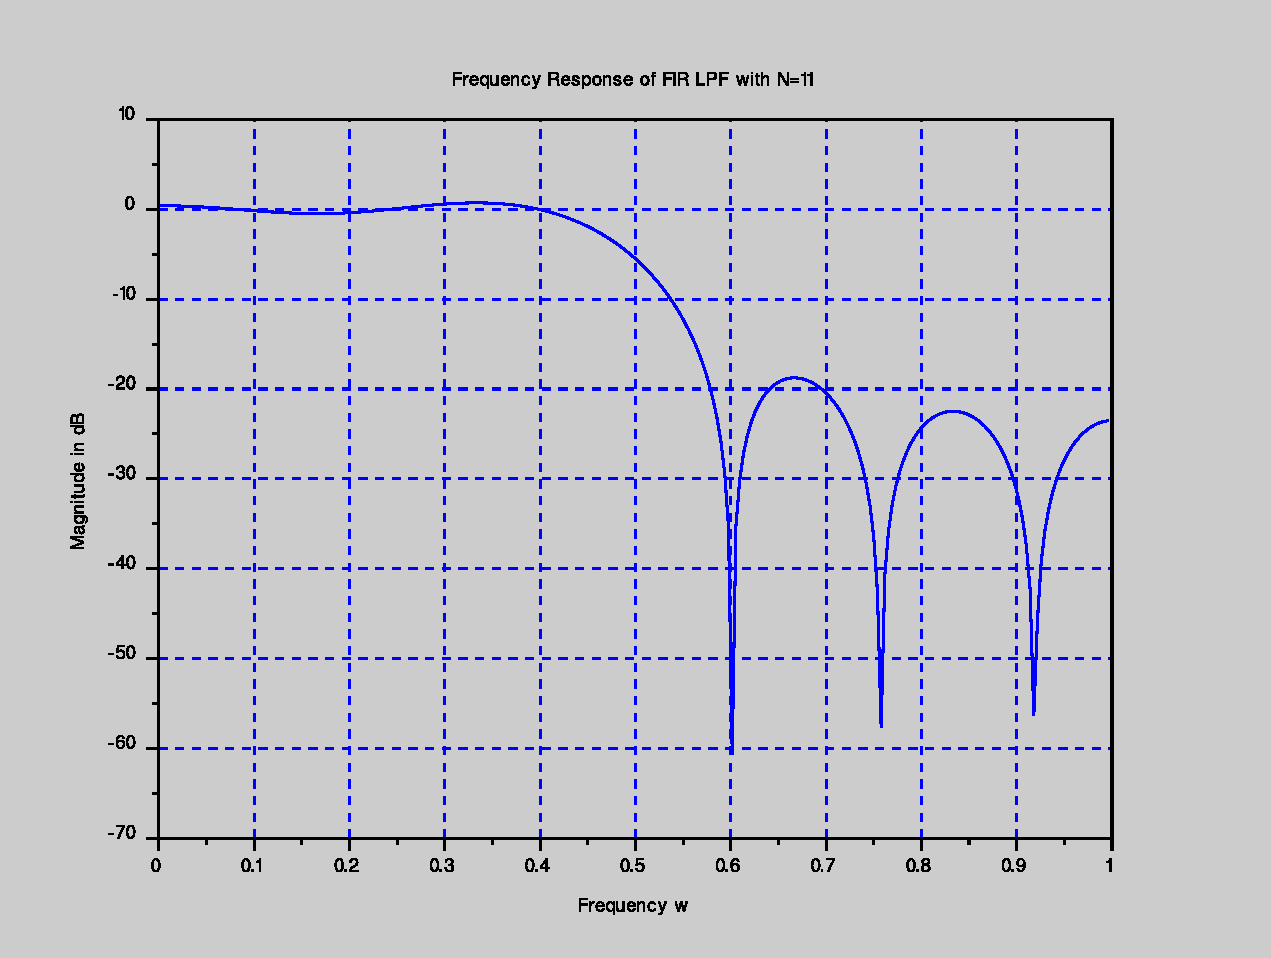
\includegraphics[scale=.5]{/home/kavya/kavyadev/DSPlab/scilabCode/firWindow.pdf}
\caption{Plot of a sequence and its DFT(magnitude and phase)}
\label{dft_sequence}
\end{figure}
